\documentclass[11pt,a4paper]{article}

\usepackage[T1]{fontenc}
\usepackage[utf8]{inputenc}
\usepackage{lmodern}
\usepackage[margin=2.5cm]{geometry}
\usepackage{graphicx}
\usepackage{amsmath}
\usepackage{booktabs}
\usepackage{xcolor}
\usepackage{float}
\usepackage{caption}
\usepackage{enumitem}
\usepackage[hidelinks]{hyperref}

% Branding Colours
\definecolor{primary}{HTML}{0F6B57}
\definecolor{scamred}{HTML}{C2312A}
\definecolor{warnamber}{HTML}{B26A00}
\definecolor{safegreen}{HTML}{1F8A4C}

\captionsetup{font=small,labelfont=bf}

\begin{document}

% -------------------------------------------------------------
% TITLE PAGE / HEADER
% -------------------------------------------------------------
\begin{titlepage}
    \centering
    \vspace*{1.5cm}
    {\LARGE \textbf{NED University of Engineering \& Technology, Karachi}\par}
    \vspace{0.4cm}
    {\large Department of Computer Science \& Software Engineering\par}
    \vspace{0.2cm}
    {\normalsize \textbf{CT-262: Introduction to Artificial Intelligence}\par}
    \vspace{2.5cm}

    {\fontsize{32}{38}\selectfont \textbf{\textcolor{primary}{Tahaffuz (تحفظ)}}\par}
    \vspace{0.4cm}
    {\Large \textbf{Explainable Expert System for Detecting Scam and Phishing Messages}\par}
    \vspace{0.3cm}
    {\normalsize \textit{Bilingual (English \& Roman Urdu) $\bullet$ MYCIN Certainty Factors $\bullet$ SWI-Prolog Engine}\par}
    \vspace{2.5cm}

    \begin{tabular}{rl}
        \textbf{Author:} & Syeda Aliza Ayaz \\
        \textbf{Roll Number:} & CT-24219 \\
        \textbf{Course Instructor:} & Sir Muhammad Wasiq Noor \\
        \textbf{Live Deployment:} & \url{https://huggingface.co/spaces/aliza-ayaz/Tahaffuz} \\
        \textbf{Date:} & \today
    \end{tabular}
    \vfill
\end{titlepage}

\newpage

% -------------------------------------------------------------
% 1. INTRODUCTION
% -------------------------------------------------------------
\section{Introduction}

Financial communication in Pakistan has rapidly transitioned to digital channels, with mobile wallets such as JazzCash and Easypaisa, as well as branchless SMS banking, serving tens of millions of citizens. However, this transition has been accompanied by an epidemic of SMS, WhatsApp, and social engineering fraud. Scammers routinely impersonate banks, telecom providers, government welfare initiatives (e.g., BISP, Ehsaas Programme), or state authorities (e.g., PTA), claiming that accounts are blocked or that cash prizes have been won.

A defining characteristic of fraudulent messaging in Pakistan is that the vast majority of scams are delivered in \textbf{Roman Urdu} (Urdu written in the Latin alphabet) or bilingual code-mixed text. Standard international email spam filters and English-only NLP models perform poorly in this environment because:
\begin{enumerate}[noitemsep]
    \item They lack vocabulary for colloquial Roman Urdu terms (e.g., \textit{foran bhejein}, \textit{inaam jeet liya}, \textit{khatoon/hazrat}).
    \item They fail to recognise local institutional contexts, such as 5-digit Pakistani official short-codes versus fraudulent 11-digit mobile phone numbers (\texttt{03xx-xxxxxxx}).
    \item Standard machine learning models operate as opaque ``black boxes'', providing binary probability outputs without explaining \textit{why} a message was flagged or giving the victim actionable guidance on what steps to take.
\end{enumerate}

\textbf{Tahaffuz} (\textit{meaning ``protection'' in Urdu}) is an explainable expert system designed to resolve these challenges. Developed strictly within the classical artificial intelligence paradigm, Tahaffuz uses rule-based knowledge representation, inexact reasoning via \textbf{MYCIN-style Certainty Factors}, and a bidirectional explanation facility implemented in \textbf{SWI-Prolog}. It evaluates input text, calculates an overall confidence score, renders a verdict (\textbf{Safe}, \textbf{Suspicious}, or \textbf{Scam}), diagnoses the underlying scam category, and provides practical advice to protect the user.

\bigskip

% -------------------------------------------------------------
% 2. EXPLANATION OF THE SYSTEM
% -------------------------------------------------------------
\section{Explanation of the System}

Tahaffuz is structured around four classical expert system pillars: a \textbf{Knowledge Base}, an \textbf{Inference Engine}, an \textbf{Explanation Facility}, and a \textbf{User Interface}.

\subsection{Architecture and Reasoning Workflow}
When a message is received by the system, it traverses four sequential processing stages:
\begin{enumerate}
    \item \textbf{Pattern and Keyword Matching (\texttt{matcher.pl}):} The raw message string is parsed against rule patterns in both English and Roman Urdu. The matcher detects indicators such as credential harvesting, lottery lures, fake helplines, urgency triggers, and suspicious URL shorteners. It actively verifies contextual negations (e.g., distinguishing between a scammer demanding an OTP versus a legitimate bank notice stating \textit{``Do not share your OTP''}).
    \item \textbf{MYCIN Uncertainty Inference (\texttt{inference.pl}):} Each indicator rule possesses an intrinsic Certainty Factor ($CF \in [0.0, 1.0]$) representing the expert's confidence in that indicator signaling fraud. Multiple firing indicators are accumulated incrementally using the classical Stanford MYCIN combination formula:
    \begin{equation}
        CF_{\text{combined}} = CF_1 + CF_2 \times (1 - CF_1)
    \end{equation}
    This formula guarantees asymptotic growth toward $1.0$ while ensuring that the order in which indicators fire does not alter the final computed score.
    \item \textbf{Decision and Safety Gating:} The aggregate confidence score is classified into standard operational bands:
    \begin{itemize}[noitemsep]
        \item $\text{Score} < 0.40$: \textcolor{safegreen}{\textbf{Safe}}
        \item $0.40 \le \text{Score} < 0.70$: \textcolor{warnamber}{\textbf{Suspicious}}
        \item $\text{Score} \ge 0.70$: \textcolor{scamred}{\textbf{Scam}} (Subject to Action Gate)
    \end{itemize}
    \textbf{The Gate Meta-Rule:} To eliminate catastrophic false alarms (such as aggressive promotional messages scoring high on urgency), a message \textit{cannot} be categorized as a \textbf{Scam} unless at least one direct ``Action Indicator'' (e.g., asking for an OTP, demanding a fee, or soliciting account credentials) has fired. Without an action indicator, high-scoring messages are conservatively capped at \textbf{Suspicious}.
    \item \textbf{Diagnosis and Decision Support (\texttt{diagnosis.pl}):} The system evaluates the fired evidence to identify the scam subtype (such as \textit{OTP / Credential Theft}, \textit{Advance-Fee Prize Scam}, or \textit{Fake Official Helpline}) and outputs safety tips advising the recipient how to respond.
\end{enumerate}

\bigskip

% -------------------------------------------------------------
% 3. MARKET USE CASE
% -------------------------------------------------------------
\section{Market Use Case}

\subsection{Target Stakeholders}
Tahaffuz provides immediate value across multiple layers of the telecommunications and financial ecosystem:
\begin{itemize}
    \item \textbf{Mobile Financial Services (MFS):} Platforms like JazzCash, Easypaisa, Nayapay, and SadaPay can integrate the lightweight expert system into their consumer smartphone apps or SMS gateways to provide real-time scam warnings before users authorize transactions.
    \item \textbf{Commercial Banks:} Customer-support call centers and online portals can deploy Tahaffuz to automatically screen suspicious messages forwarded by banking customers.
    \item \textbf{Telecommunications Operators and Regulators (PTA):} Telecom providers (Jazz, Telenor, Zong, Ufone) can utilize the rule engine at the SMSC (Short Message Service Center) level to filter broadcast smishing campaigns without requiring heavy GPU infrastructure.
    \item \textbf{General Consumers \& Vulnerable Populations:} Everyday citizens, particularly those with low digital literacy or who communicate primarily in Roman Urdu, receive immediate, understandable explanations in plain language rather than opaque technical warnings.
\end{itemize}

\subsection{Key Competitive Advantages}
\begin{itemize}
    \item \textbf{Zero GPU Dependency \& Lightweight Execution:} Unlike multi-billion parameter LLMs, the SWI-Prolog engine evaluates rules in less than 5 milliseconds, consuming negligible memory and running on low-cost servers or edge devices.
    \item \textbf{Auditability and Regulatory Compliance:} Banks and compliance officers require full transparency. Because every rule has a deterministic trace, verdicts are 100\% defensible and verifiable.
    \item \textbf{Rapid Knowledge Adaptation:} When scammers invent a new keyword pattern (e.g., a new government subsidy scheme), domain experts can update the knowledge base with a single rule declaration in minutes, requiring zero model retraining or dataset re-labeling.
\end{itemize}

\bigskip

% -------------------------------------------------------------
% 4. SCREENSHOTS OF THE PROJECT
% -------------------------------------------------------------
\section{Screenshots of the Project}

The application interface was deployed with both an interactive web dashboard and a cloud-hosted Gradio platform. Figures~\ref{fig:home}--\ref{fig:safe} demonstrate the behavior of the system across standard test cases.

\begin{figure}[H]
    \centering
    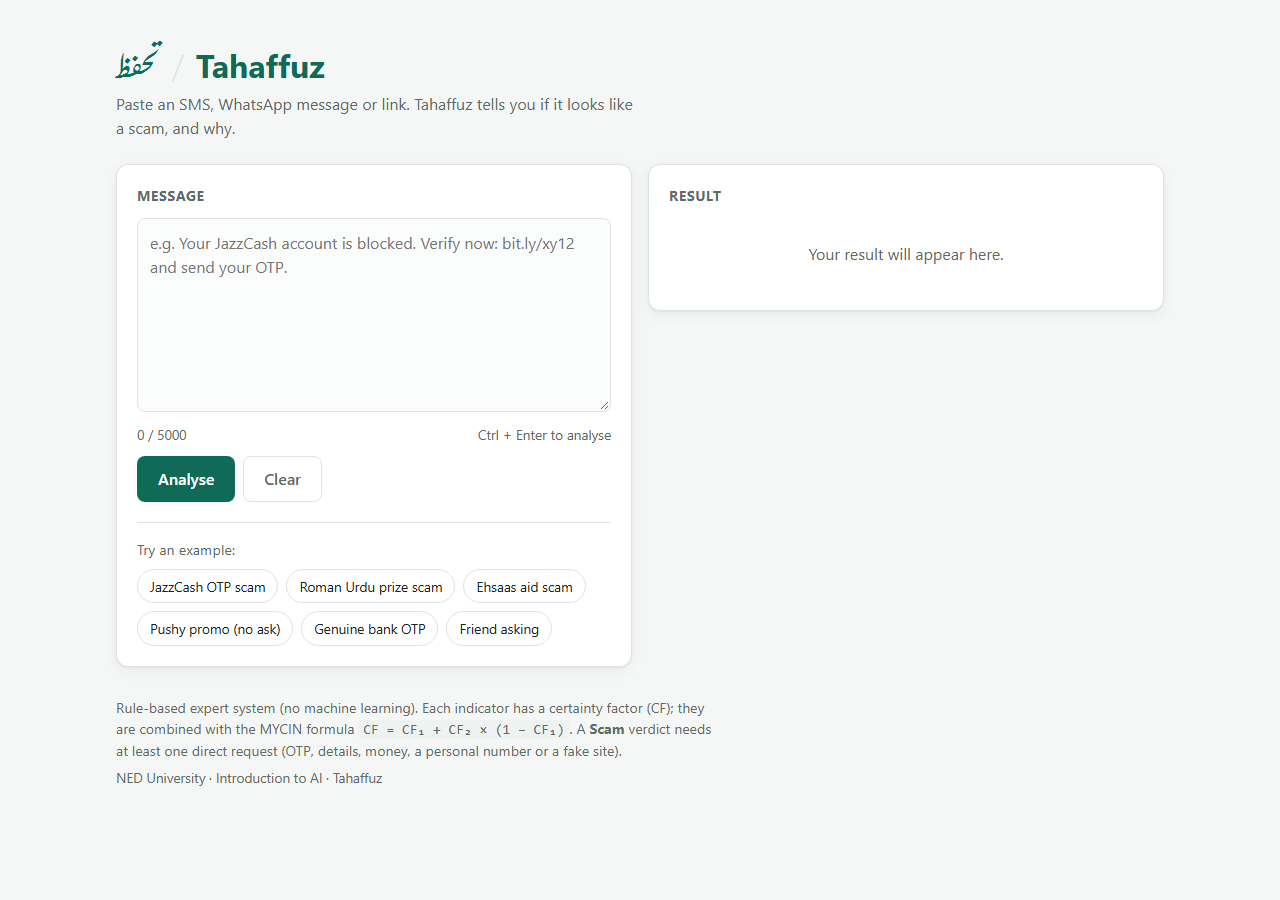
\includegraphics[width=0.88\linewidth]{figures/ss_home.png}
    \caption{Tahaffuz Dashboard: Message input area, clickable example templates, and initial state.}
    \label{fig:home}
\end{figure}

\begin{figure}[H]
    \centering
    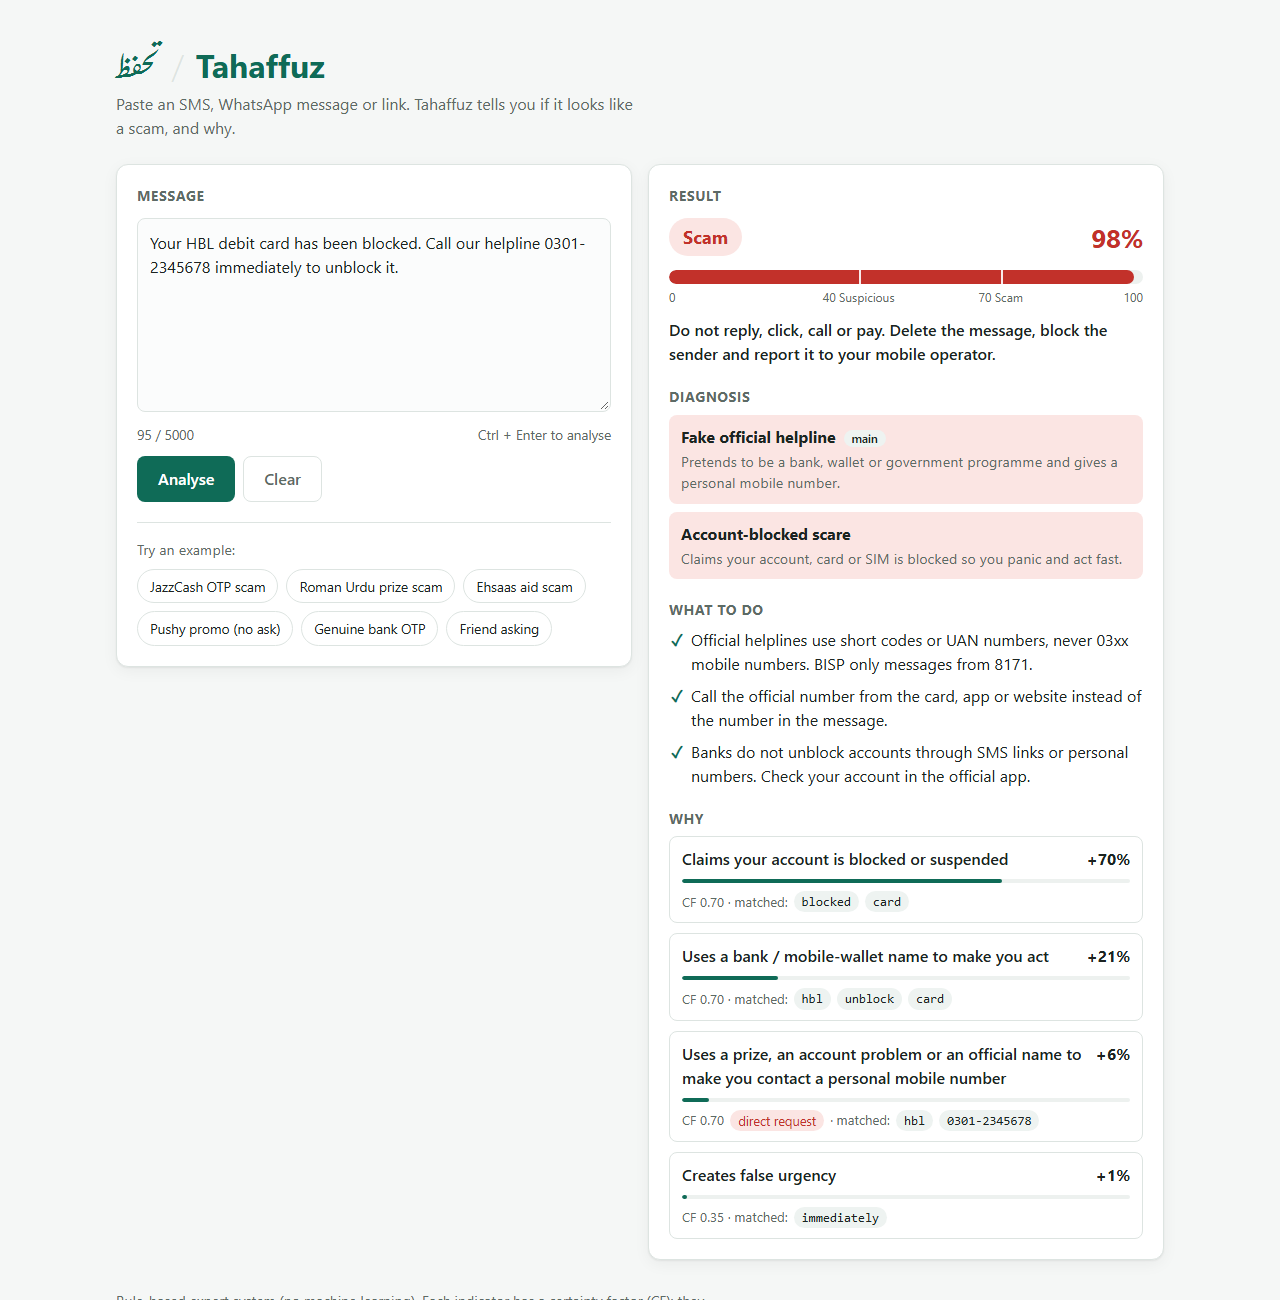
\includegraphics[width=0.88\linewidth]{figures/ss_scam.png}
    \caption{\textbf{Scam Verdict (98\% Confidence):} Fake HBL helpline scam. The system identifies the scam type (\textit{Fake official helpline}, \textit{Account-blocked scare}), provides clear protective advice, and breaks down the exact CF contribution of each matched keyword.}
    \label{fig:scam}
\end{figure}

\begin{figure}[H]
    \centering
    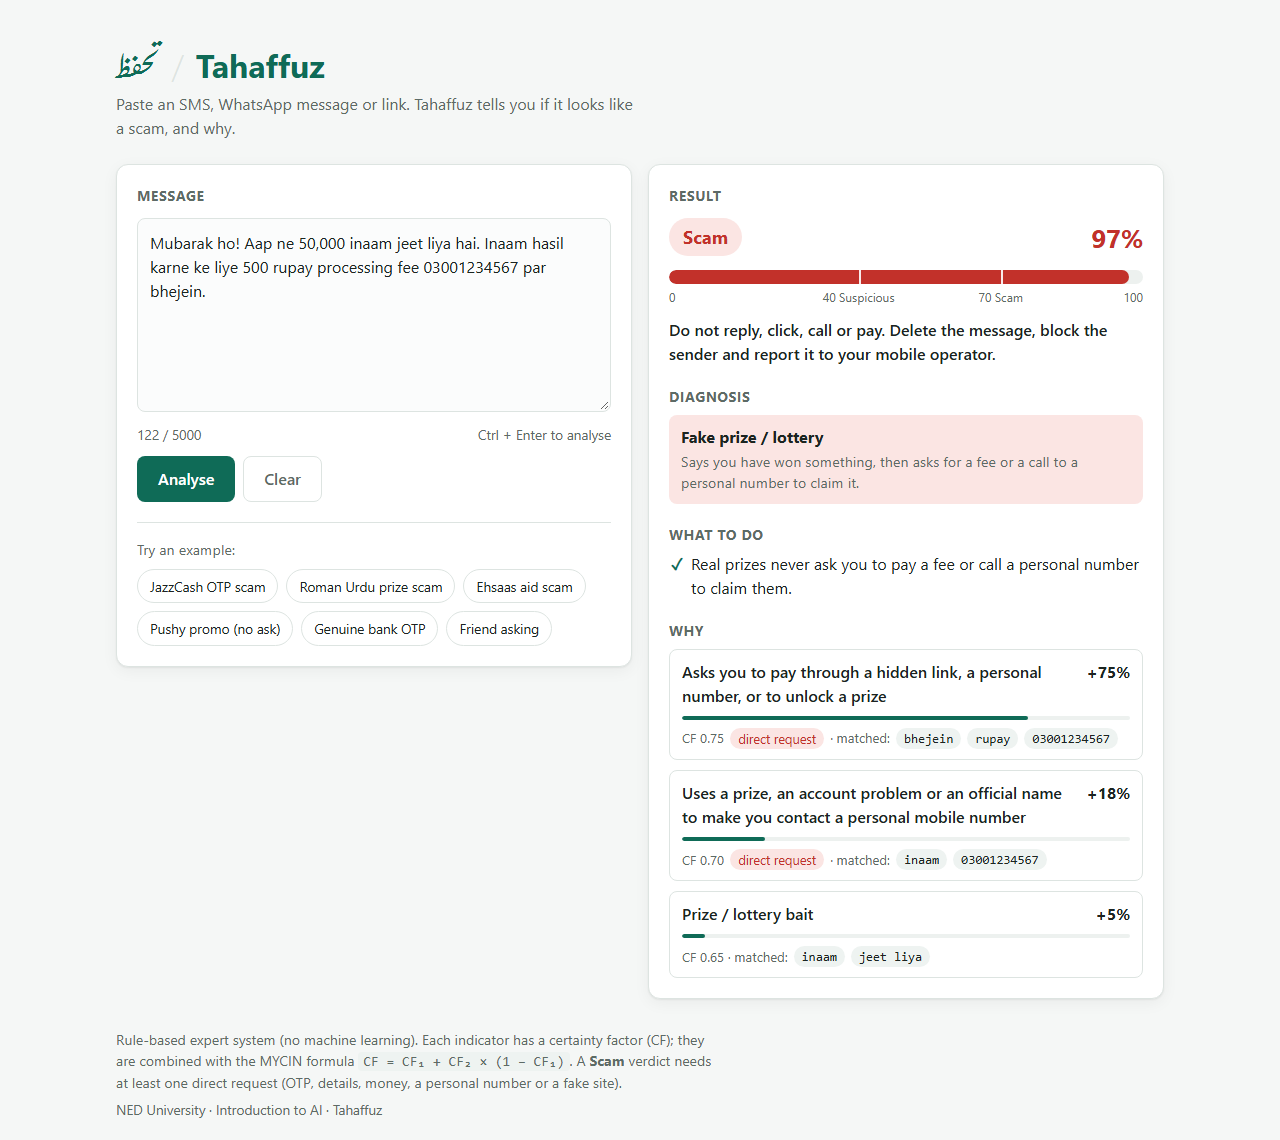
\includegraphics[width=0.88\linewidth]{figures/ss_roman.png}
    \caption{\textbf{Roman Urdu Scam (97\% Confidence):} Identifies lottery prize deception (\textit{inaam jeet liya}, \textit{processing fee}, \textit{0300... personal mobile number}). Diagnosed as \textit{Fake prize / lottery}.}
    \label{fig:roman}
\end{figure}

\begin{figure}[H]
    \centering
    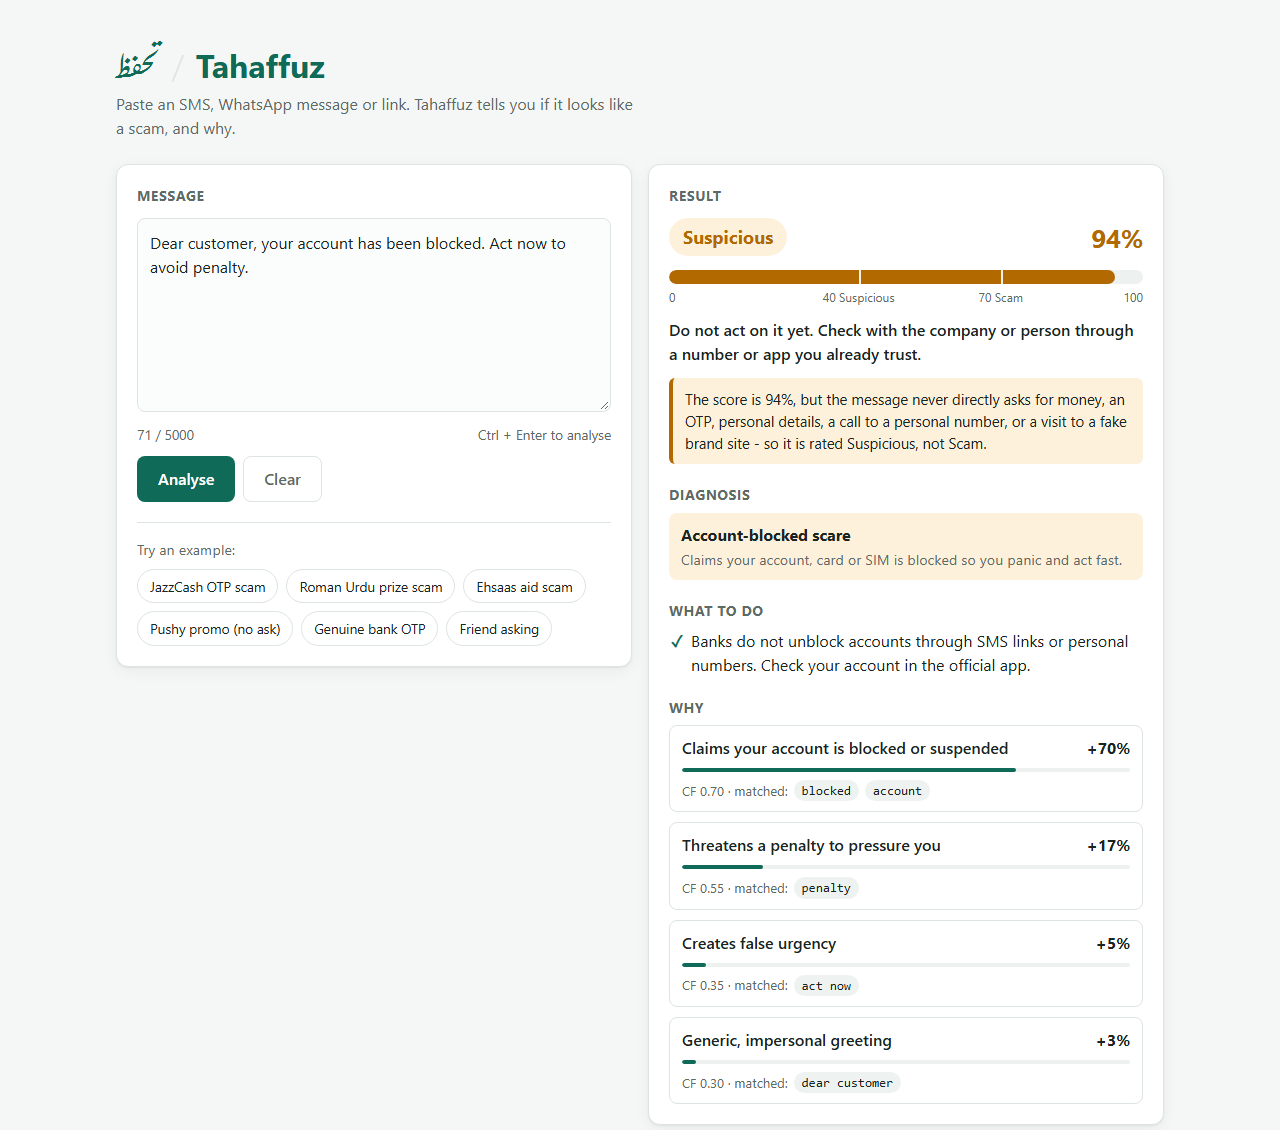
\includegraphics[width=0.88\linewidth]{figures/ss_suspicious.png}
    \caption{\textbf{The Gate Meta-Rule in Action (Suspicious at 94\%):} The message contains aggressive urgency and an account threat, but because it contains no direct call-to-action (no link, no request for funds or OTP), the verdict is capped at \textbf{Suspicious} to avoid a false positive.}
    \label{fig:suspicious}
\end{figure}

\begin{figure}[H]
    \centering
    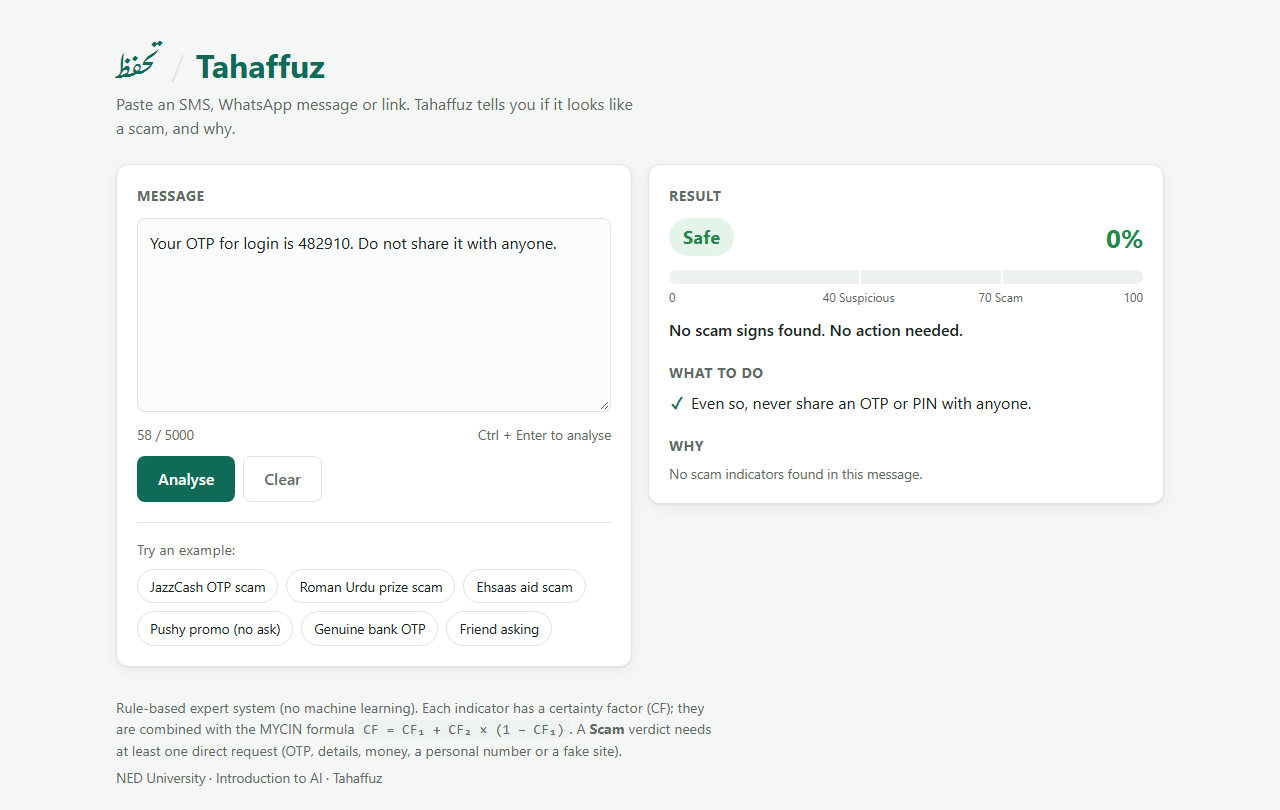
\includegraphics[width=0.88\linewidth]{figures/ss_safe.png}
    \caption{\textbf{Safe Verdict (0\% Confidence):} Genuine bank OTP message. The negation engine detects \textit{``Do not share it with anyone''}, preventing the OTP-theft indicator from falsely firing.}
    \label{fig:safe}
\end{figure}

\end{document}

